\begin{frame}{Integrative Modelling Platform}
    Now we already know what is IMP. It is computationally expensive and time consuming due Markov Chain Monte Carlo (MCMC) sampling. \\
    \bigskip
    \pause
    We wish to replace the computationally expensive sampling techniques to paradigms used in DREAM: \\
    \begin{itemize}
        \item Orientate the structures of subunits based on experimental evidence which is similar to substruture computation in DREAM
        \item Register the subunits in one shot while respecting the experimental evidence. (an enhancement of DREAM's registration)
    \end{itemize}
\end{frame}

\begin{frame}{How will this happen ?}
    \begin{itemize}
        \item Our substructures in this case are different kinds of proteins. \\
        \item We have cross-links data available these proteins. \\
    \end{itemize}

    Given this information, we need to do one shot registration of these proteins to model the structure of complex.

\end{frame}

\begin{frame}{}
    \begin{figure}
        \centering
        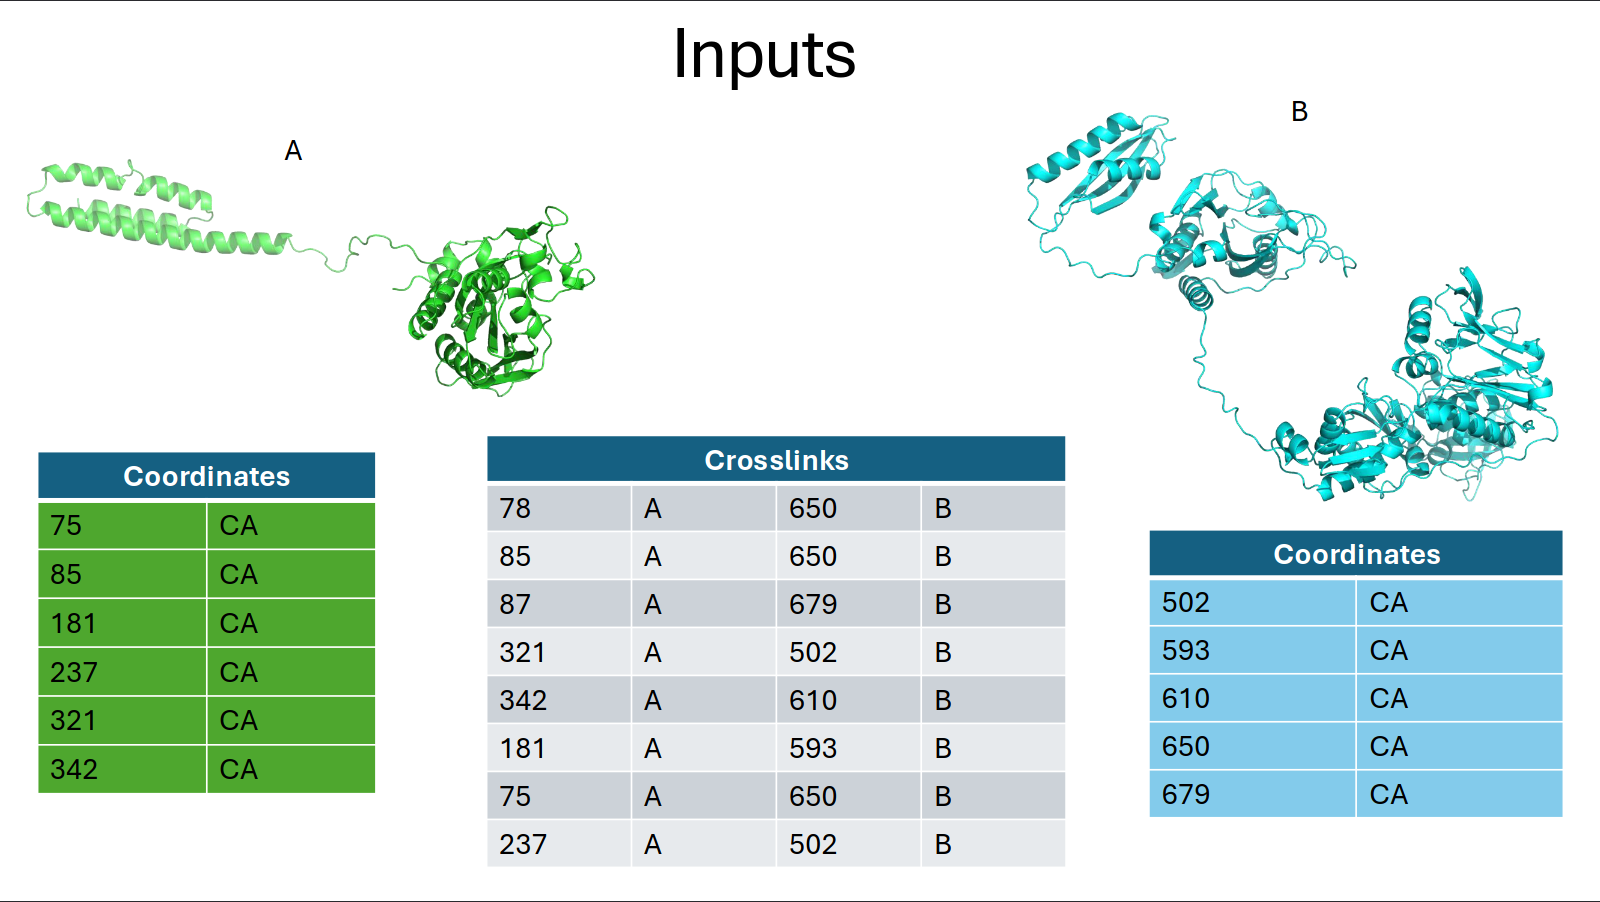
\includegraphics[width=1\textwidth]{images/local.png}
        \caption{Example of 2 proteins with cross-links data}
        \label{fig:my_label}
    \end{figure}
\end{frame}

\begin{frame}{Problem}
    \begin{figure}
        \centering
        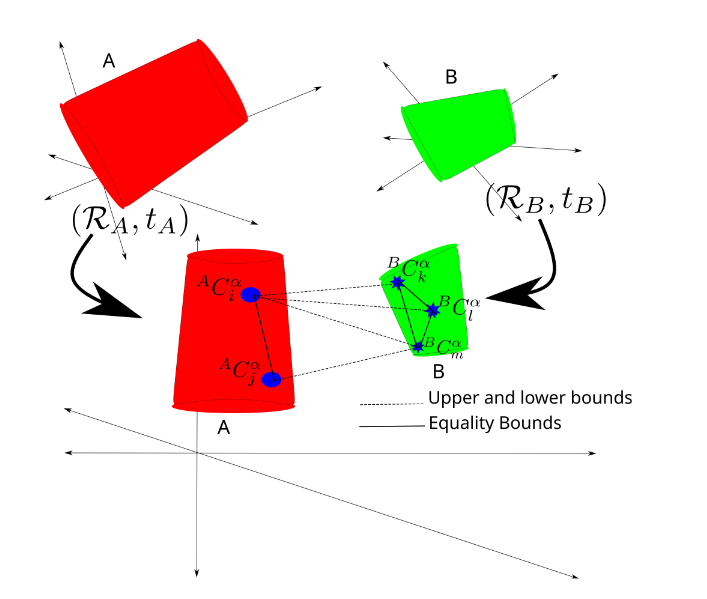
\includegraphics[width=0.7\textwidth]{images/toy1.png}
        \caption{Consider A,B as proteins and the lines as cross-links}
        \label{fig:my_label}
    \end{figure}
\end{frame}

\begin{frame}{Solution}
    \begin{figure}
        \centering
        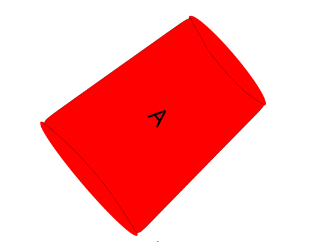
\includegraphics[width=0.3\textwidth]{images/A.png}
        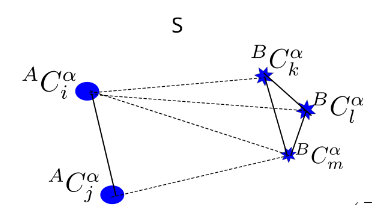
\includegraphics[width=0.3\textwidth]{images/S.png}
        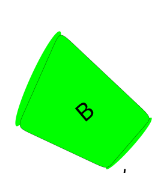
\includegraphics[width=0.3\textwidth]{images/B.png}
        \label{fig:my_label}
    \end{figure}
    Consider S as hypothetical framework. 
    \pause
    Then we can do one shot registration of A,S and B
\end{frame}

\begin{frame}{Solution}
    \begin{figure}
        \centering
        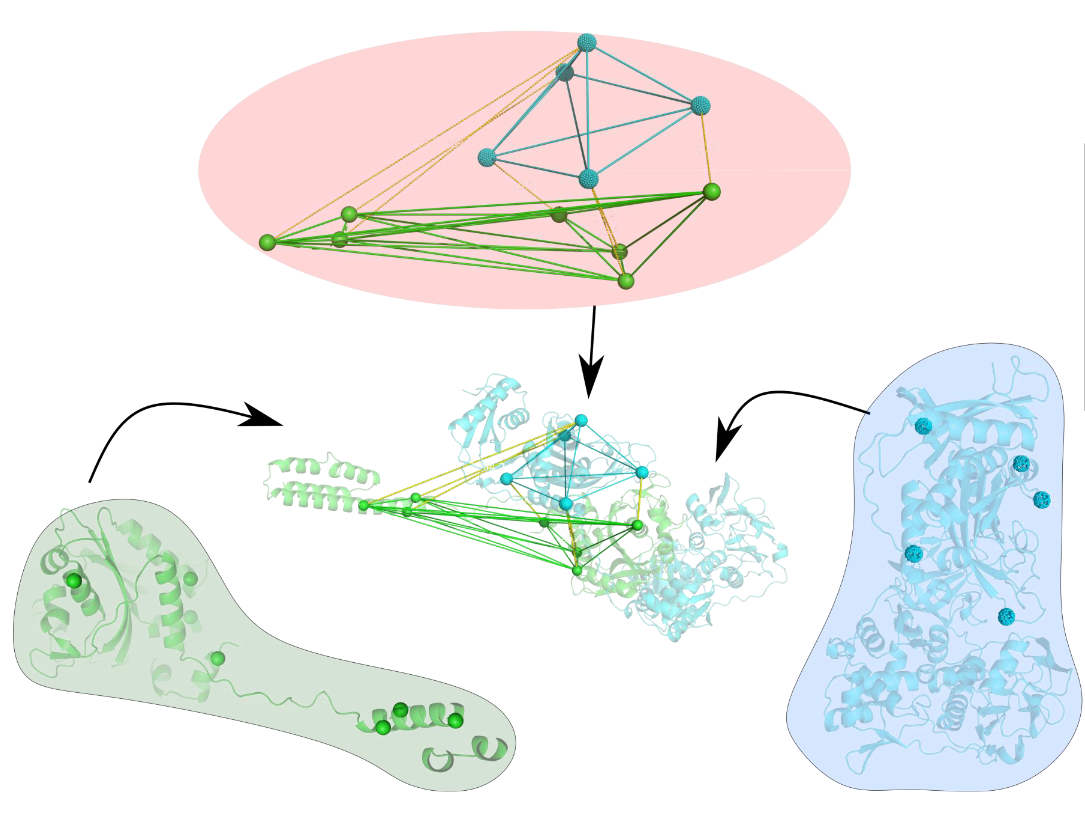
\includegraphics[width=0.7\textwidth]{images/final.png}
        \caption{One shot registration}
        \label{fig:my_label}
    \end{figure}
\end{frame}

\begin{frame}{Some Observations}
    1. In the hypothetical framework, we have all pairs of distances between C-alpha atoms in each protein. \\
    \pause
    2. For registering n proteins, only 1 hypothetical fragment is needed. So registration of $n+1$ proteins is done. \\
\end{frame}

\begin{frame}{Implementation}
    Consider the case of "1dfj" which has E and I chain. We have crosslink data available. Here is the true structure:

    \begin{figure}
        \centering
        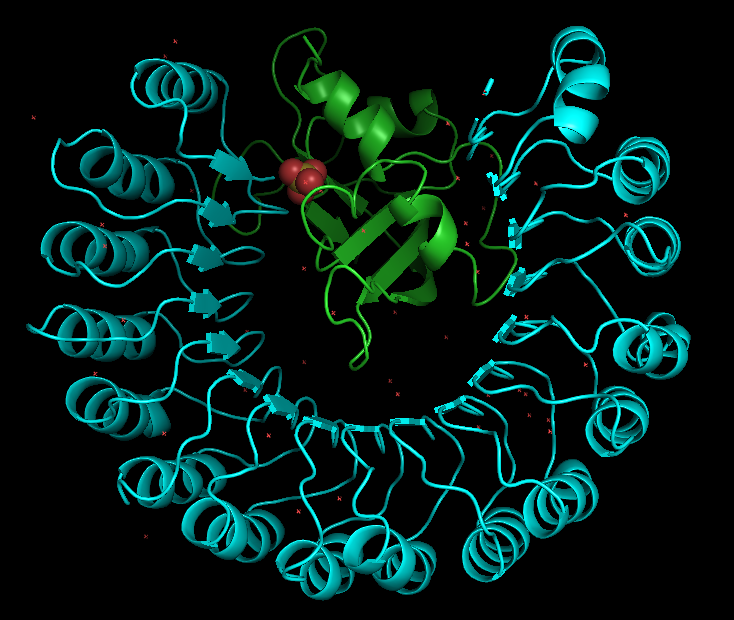
\includegraphics[width=0.5\textwidth]{images/1dfj_1.png}
        \caption{True structure of 1dfj}
        \label{fig:my_label}
    \end{figure}
    
\end{frame}

\begin{frame}{Structure obtained using our method}
    \begin{figure}
        \centering
        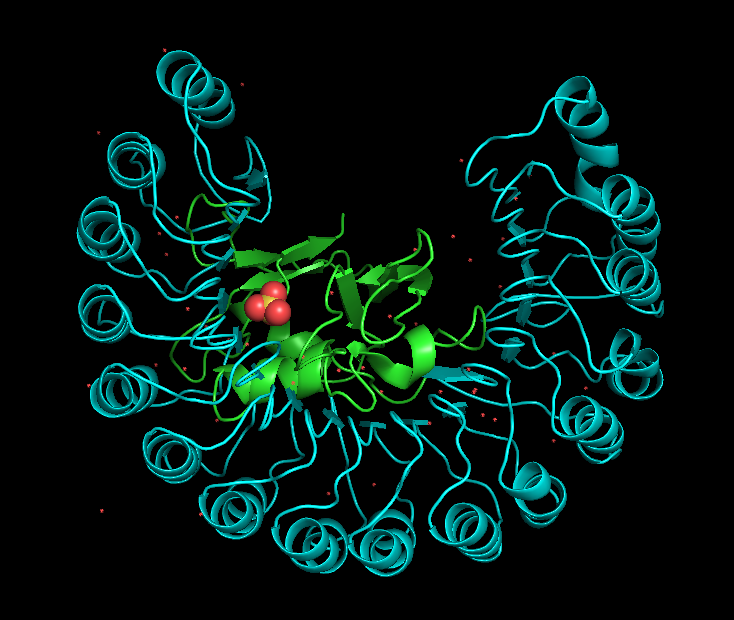
\includegraphics[width=0.5\textwidth]{images/1dfj_2.png}
        \caption{Structure obtained using our method}
        \label{fig:my_label}
    \end{figure}

    \pause

    There are 2 problems:
    \begin{enumerate}
        \item Clashes between proteins
        \item Flipped Ramachandran angles
    \end{enumerate}
\end{frame}

\begin{frame}{Possible Fix for Clashes}
    Take random subset of crosslink data instead of all crosslink data. Here is the result for random subset of 6 crosslinks out of 12:

    \begin{figure}
        \centering
        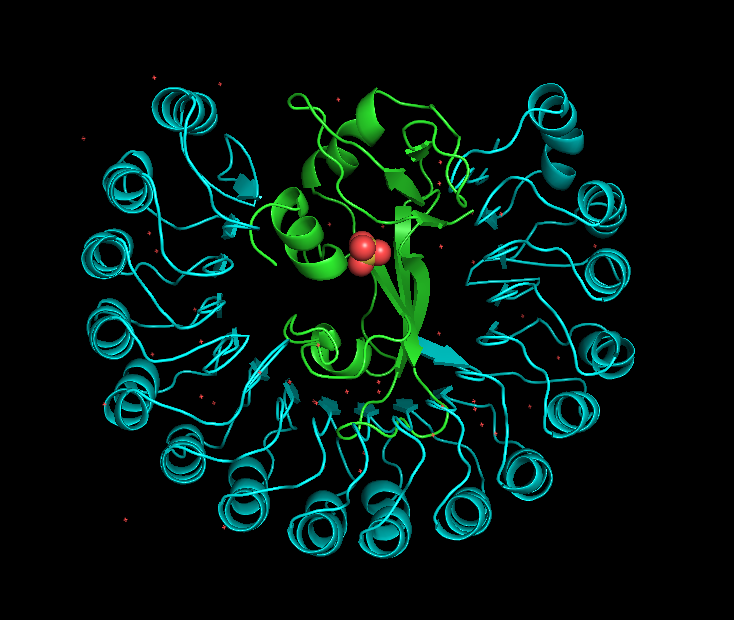
\includegraphics[width=0.5\textwidth]{images/1dfj_3.png}
    \end{figure}
    
    Again there is flipped Ramachandran angles, but clashes have reduced.
\end{frame}

\begin{frame}{Next Steps}
    1. Fix the flipped Ramachandran angles \\
    2. If this does not work, then translate to remove the clash keeping the orientation same \\
    3. Energy minimization \\

    \bigskip

    In this way we are taking experimental data into consideration instead of random sampling of initial configurations.
\end{frame}

\begin{frame}{Energy Minimization}
    \begin{figure}
        \centering
        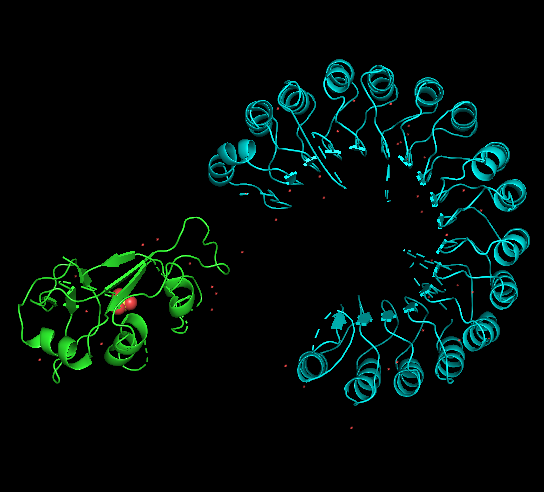
\includegraphics[width=0.5\textwidth]{images/1dfj_4.png}
        \caption{Translating with same orientation}
        \label{fig:my_label}
    \end{figure}

    Now we run Energy minimization to get the final structure, which will satisy the given experimental (crosslink) data.
\end{frame}